\documentclass[10pt, a4paper]{article}

\usepackage{ctex}
\usepackage{xeCJK}
\usepackage{caption}
\usepackage{geometry}
\geometry{
    left = 0.6in,
    right = 0.6in,
    top = 0.8in,
    bottom = .6in
}
\usepackage{amssymb}
\usepackage{amsbsy}
\usepackage{amsmath}
\usepackage{xcolor}
\usepackage{mathrsfs}
\usepackage{graphicx}
\usepackage{pifont}
\usepackage{tikz}
\usepackage{tasks}
\settasks{
    label = \textcolor{purple}{\Alph*.},
    label-width = 14pt
}
\pagestyle{empty}

\newcommand{\Title}[3]{
    \begin{center}
        \Large \textbf{中国电子学会 #1~年~#2~月 Scratch~#3级考试}
    \end{center}
}
\newcommand{\TimeAndName}[1]{
    \begin{center}
        考试时间:~#1~ 分钟 \qquad\qquad\qquad\qquad 姓名:\underline{\quad\quad\quad\quad}
    \end{center}
}
\newcommand{\hq}{\hfill(\qquad)}

\begin{document}
    \Title{2023}{05}{三} % 标题
    \TimeAndName{60} % 考试时间及姓名

    % 单选题
    \vspace{2mm}
    {\noindent\textbf{第一部分、单选题(共 25 题,每题 2 分,共50分.)}}
    \begin{enumerate}
        % 1
        \item 关于变量,下列描述错误的是? \hq
        \begin{tasks}(4)
            \task 只能建一个变量
            \task 变量可以隐藏
            \task 变量可以删除
            \task 变量的值可以修改
        \end{tasks}

        % 2
        \item 运行下列程序后,变量“和”的值是?\hq
        \begin{tasks}(4)
            \task 1
            \task 4
            \task 5
            \task 6
        \end{tasks}

        \begin{figure}[htbp]
            \centering
            \begin{minipage}[t]{.12\textwidth}
                \centering
                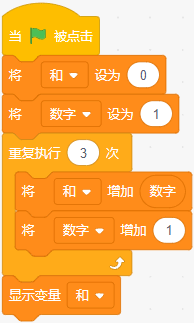
\includegraphics[width=\textwidth]{figure/2.png}
                \caption*{第 2 题}
            \end{minipage}
            \begin{minipage}[t]{.25\textwidth}
                \centering
                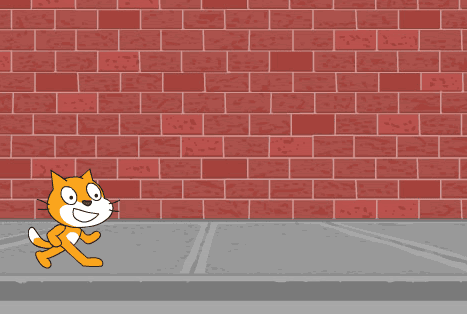
\includegraphics[width=\textwidth]{figure/4.png}
                \caption*{第 4 题}
            \end{minipage}
            \begin{minipage}[t]{.33\textwidth}
                \centering
                \begin{minipage}[t]{.63\textwidth}
                    \centering
                    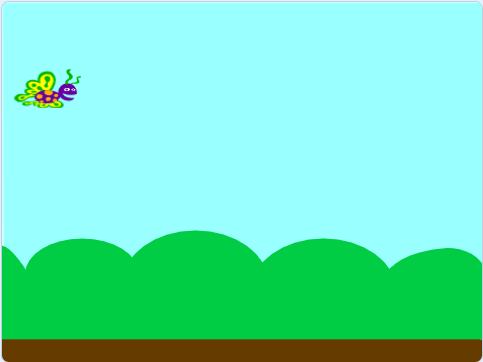
\includegraphics[width=\textwidth]{figure/5-1.png}
                \end{minipage}
                \begin{minipage}[t]{.32\textwidth}
                    \centering
                    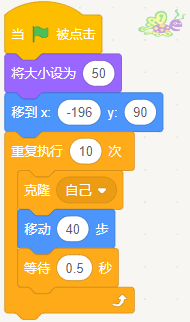
\includegraphics[width=\textwidth]{figure/5-2.png}
                \end{minipage}
                \caption*{第 5 题}
            \end{minipage}
            \begin{minipage}[t]{.23\textwidth}
                \centering
                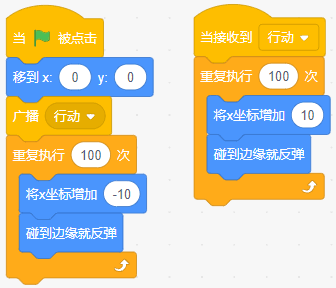
\includegraphics[width=\textwidth]{figure/6.png}
                \caption*{第 6 题}
            \end{minipage}
        \end{figure}

        % 3
        \item 当前角色的造型如下图所示,运行程序后,最后停留在哪个造型上? \hq
        
        \begin{minipage}{.35\textwidth}
            \centering
            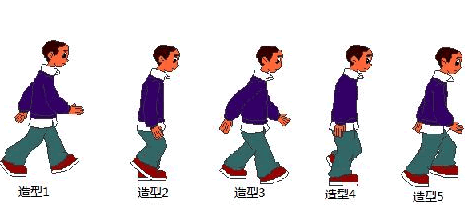
\includegraphics[width=\textwidth]{figure/3-1.png}
        \end{minipage}
        \begin{minipage}{.15\textwidth}
            \centering
            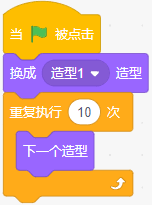
\includegraphics[width=.7\textwidth]{figure/3-2.png}
        \end{minipage}
        \begin{minipage}{.4\textwidth}
            \centering
            \begin{tasks}(2)
                \task 造型1
                \task 造型2
                \task 造型3
                \task 造型5
            \end{tasks}
        \end{minipage}

        % 4
        \item 下列哪个选项可以实现小猫从左跑到右,碰到舞台边缘停止前进,面向左边方向?\hq
        \begin{tasks}(4)
            \task 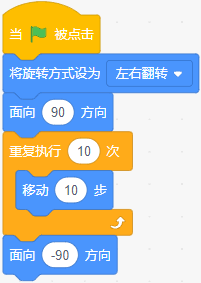
\includegraphics[width=.12\textwidth]{figure/4a.png}
            \task 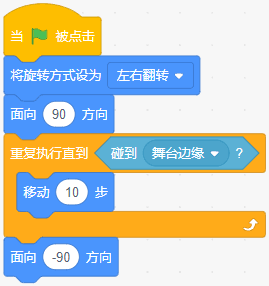
\includegraphics[width=.16\textwidth]{figure/4b.png}
            \task 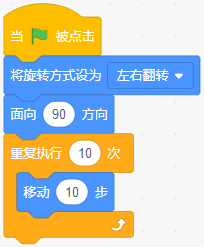
\includegraphics[width=.14\textwidth]{figure/4c.png}
            \task 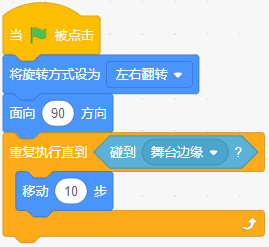
\includegraphics[width=.18\textwidth]{figure/4d.png}
        \end{tasks}

        % 5
        \item 蝴蝶程序如右图所示,点击绿旗,程序运行后,最终看到几只蝴蝶? \hq
        \begin{tasks}(4)
            \task 1只
            \task 9只
            \task 10只
            \task 11只
        \end{tasks}

        % 6
        \item 默认小猫角色,点击绿旗,运行程序后,下列描述正确的是?\hq
        \begin{tasks}
            \task 小猫先向右移动,碰到舞台边缘反弹向左移动;再次碰到边缘后,向右移动;重复100次,最后停下来
            \task 小猫先向左移动,碰到舞台边缘反弹向右移动;再次碰到边缘后,向左移动;重复100次,最后停下来
            \task 小猫保持原地不动
            \task 小猫忽左忽右地在舞台中移动,碰到边缘反弹,继续忽左忽右地运动
        \end{tasks}

        \newpage
        % 7
        \item 以广播的形式控制角色向前移动,下列哪个选项最合适?\hq
        \begin{tasks}(4)
            \task 123456
            \task @\#\%\^{}
            \task 前进
            \task ABC
        \end{tasks}

        % 8
        \item 淘气的生日是12月份的某一天,下列哪个选项一定能生成这一天?\hq
        \begin{tasks}(4)
            \task 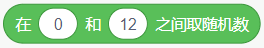
\includegraphics[width=.18\textwidth]{figure/8a.png}
            \task 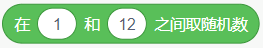
\includegraphics[width=.18\textwidth]{figure/8b.png}
            \task 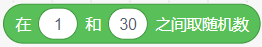
\includegraphics[width=.18\textwidth]{figure/8c.png}
            \task 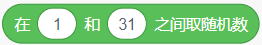
\includegraphics[width=.18\textwidth]{figure/8d.png}
        \end{tasks}

        % 9
        \item 小猫在舞台中心,面向90度方向,运行程序后,下列选项正确的是?\hq
        \begin{tasks}(2)
            \task 小猫距离舞台中心最少9步
            \task 小猫距离舞台中心最少15步
            \task 小猫距离舞台中心最多3步
            \task 小猫距离舞台中心最多5步
        \end{tasks}

        \begin{figure}[htbp]
            \centering
            \begin{minipage}[t]{.25\textwidth}
                \centering
                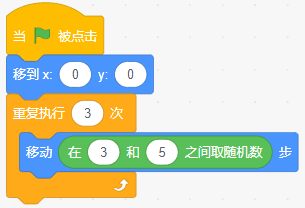
\includegraphics[width=\textwidth]{figure/9.png}
                \caption*{第 9 题}
            \end{minipage}
            \begin{minipage}[t]{.13\textwidth}
                \centering
                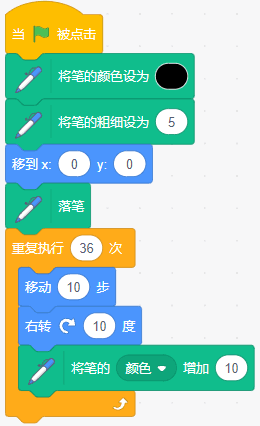
\includegraphics[width=\textwidth]{figure/10.png}
                \caption*{第 10 题}
            \end{minipage}
            \begin{minipage}[t]{.28\textwidth}
                \centering
                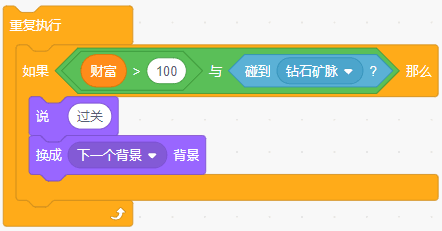
\includegraphics[width=\textwidth]{figure/13.png}
                \caption*{第 13 题}
            \end{minipage}
            \begin{minipage}[t]{.11\textwidth}
                \centering
                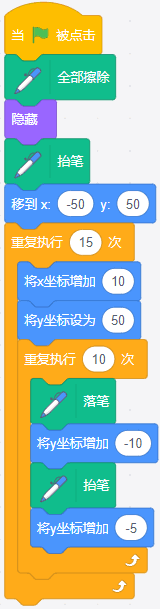
\includegraphics[width=\textwidth]{figure/14.png}
                \caption*{第 14 题}
            \end{minipage}
        \end{figure}

        % 10
        \item 运行下列程序后,画出的图形是?\hq
        \begin{tasks}(4)
            \task 
\includegraphics[width=.08\textwidth]{figure/10a.png}
            \task 
\includegraphics[width=.08\textwidth]{figure/10b.png}
            \task 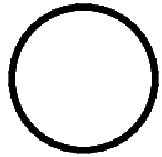
\includegraphics[width=.08\textwidth]{figure/10c.png}
            \task 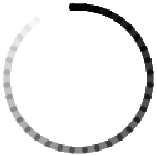
\includegraphics[width=.08\textwidth]{figure/10d.png}
        \end{tasks}

        % 11
        \item 关于“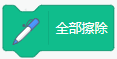
\includegraphics[width=.1\textwidth]{figure/11.png}”积木,下列描述正确的是?\hq
        \begin{tasks}(2)
            \task 只能擦除画笔所画的图形
            \task 只能擦除图章和画笔所画的图形
            \task 可以擦除背景
            \task 可以擦除画笔、图章所绘的的图形及背景
        \end{tasks}

        % 12
        \item 关于“广播”,下列描述正确的是?\hq
        \begin{tasks}(2)
            \task 广播只能由角色发出
            \task 广播的内容可以是字符或数值,但不能是变量
            \task 舞台不能发送广播,但可以接收广播
            \task 广播可以被任何角色以及舞台接收
        \end{tasks}

        % 13
        \item 运行程序后,下列描述正确的是?\hq
        \begin{tasks}(2)
            \task 财富值大于100就过关
            \task 找到钻石矿脉就过关
            \task 财富值大于100,或者找到钻石矿脉都可以过关
            \task 财富值大于100,且同时找到钻石矿脉才能过关
        \end{tasks}
        
        % 14
        \item 运行下列程序后,画出的图形是?\hq
        \begin{tasks}(4)
            \task 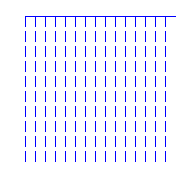
\includegraphics[width=.08\textwidth]{figure/14a.png}
            \task 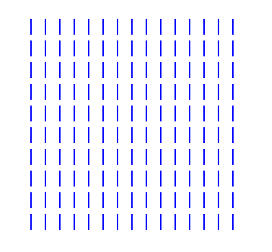
\includegraphics[width=.08\textwidth]{figure/14b.png}
            \task 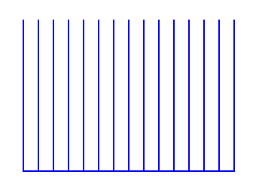
\includegraphics[width=.1\textwidth]{figure/14c.png}
            \task 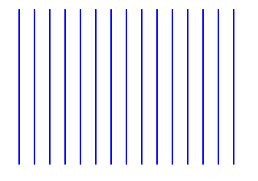
\includegraphics[width=.1\textwidth]{figure/14d.png}
        \end{tasks}

        \newpage
        % 15
        \item 小动物们排队做早操,第一排有1个小动物,第二排有3个小动物,第三排有5个小动物,以此类推$\cdots$排了8排,算一算一共有多少个小动物?\hq
        \begin{tasks}(4)
            \task 24个
            \task 32个
            \task 64个
            \task 128个
        \end{tasks}

        % 16
        \item 运行下列程序后,变量 $a$ 和变量 $b$ 之间的关系是?\hq
        
        \begin{minipage}{.4\textwidth}
            \centering
            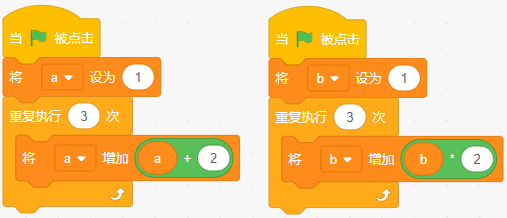
\includegraphics[width=.8\textwidth]{figure/16.png}
        \end{minipage}
        \begin{minipage}{.5\textwidth}
            \begin{tasks}(2)
                \task $a>b$
                \task $a<b$
                \task $a=b$
                \task $a$是$b$的2倍
            \end{tasks}
        \end{minipage}
        

        % 17
        \item 骰子角色有6个造型,分别对应1$\sim$ 6点,下列哪个选项不能让骰子角色换成随机的造型?\hq
        \begin{tasks}(4)
            \task 
\includegraphics[width=.17\textwidth]{figure/17a.png}
            \task 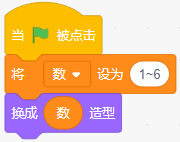
\includegraphics[width=.12\textwidth]{figure/17b.png}
            \task 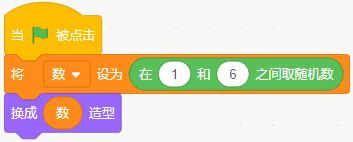
\includegraphics[width=.18\textwidth]{figure/17c.png}
            \task 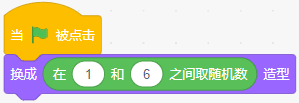
\includegraphics[width=.18\textwidth]{figure/17d.png}
        \end{tasks}

        % 18
        \item 下列哪段程序能够计算出100以内所有双数的和,并将结果存到变量sum里?\hq
        \begin{tasks}(4)
            \task 
\includegraphics[width=.12\textwidth]{figure/18a.png}
            \task 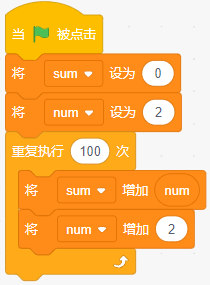
\includegraphics[width=.12\textwidth]{figure/18b.png}
            \task 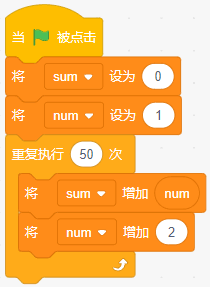
\includegraphics[width=.12\textwidth]{figure/18c.png}
            \task 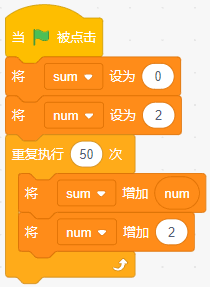
\includegraphics[width=.12\textwidth]{figure/18d.png}
        \end{tasks}

        % 19
        \item 楼道的声控灯会在有响声的时候亮起,等5秒以后熄灭,下列哪个选项可以实现这个功能?\hq
        \begin{tasks}(4)
            \task 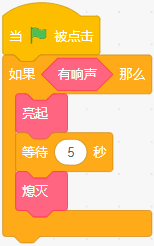
\includegraphics[width=.11\textwidth]{figure/19a.png}
            \task 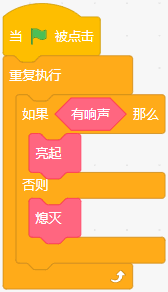
\includegraphics[width=.1\textwidth]{figure/19b.png}
            \task 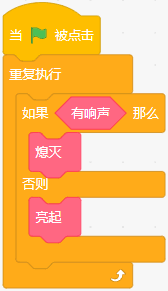
\includegraphics[width=.1\textwidth]{figure/19c.png}
            \task 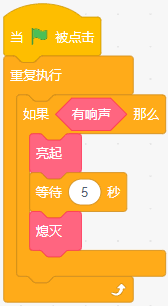
\includegraphics[width=.1\textwidth]{figure/19d.png}
        \end{tasks}

        % 20
        \item 迷宫地图如下图所示,机器人只能走蓝、绿、黄色方格,找到钻石,每一格的长度是50步,下列哪个选项不能让机器人拿到宝石?\hq
        
        \begin{minipage}{.2\textwidth}
            \centering
            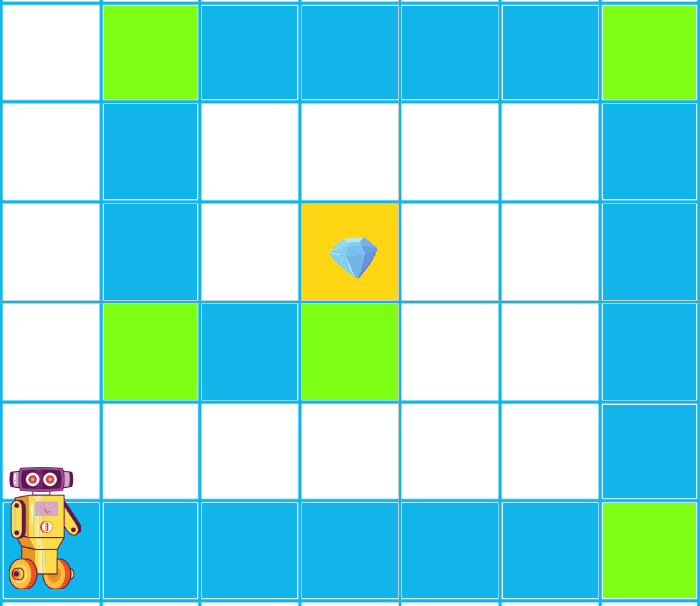
\includegraphics[width=\textwidth]{figure/20.png}
        \end{minipage}
        \begin{minipage}{.73\textwidth}
            \begin{tasks}(4)
                \task 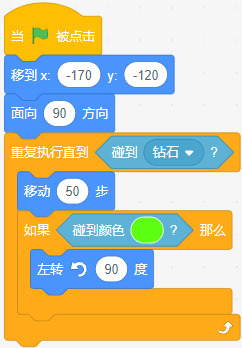
\includegraphics[width=.18\textwidth]{figure/20a.png}
                \task 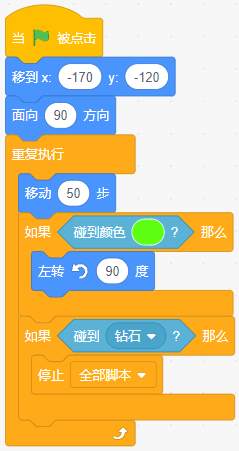
\includegraphics[width=.14\textwidth]{figure/20b.png}
                \task 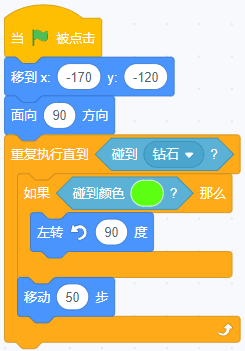
\includegraphics[width=.18\textwidth]{figure/20c.png}
                \task 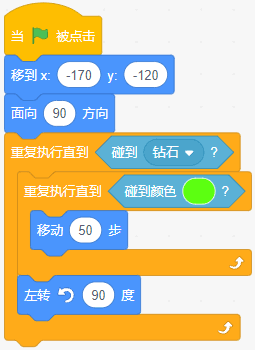
\includegraphics[width=.18\textwidth]{figure/20d.png}
            \end{tasks}
        \end{minipage}

        % 21
        \item 下列哪个选项可以画出右图所示的图案?\hq
        
        \begin{minipage}{.2\textwidth}
            \centering
            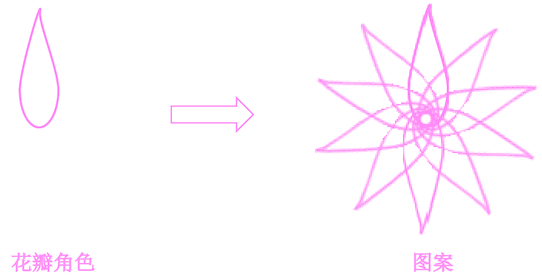
\includegraphics[width=\textwidth]{figure/21.png}
        \end{minipage}
        \begin{minipage}{.73\textwidth}
            \begin{tasks}(4)
                \task 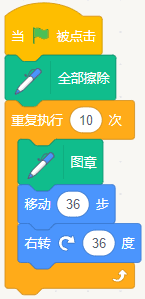
\includegraphics[width=.15\textwidth]{figure/21a.png}
                \task 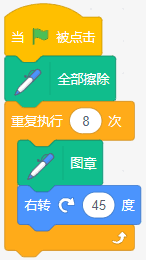
\includegraphics[width=.18\textwidth]{figure/21b.png}
                \task 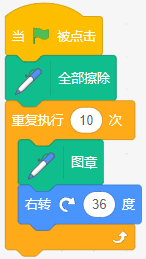
\includegraphics[width=.18\textwidth]{figure/21c.png}
                \task \includegraphics[width=.18\textwidth]{figure/21d.png}
            \end{tasks}
        \end{minipage}

        \newpage
        % 22
        \item 制作一个打砖块小游戏,下列哪个选项能实现克隆出一排6块砖块? \hq
        \begin{tasks}(4)
            \task \includegraphics[width=.18\textwidth]{figure/22a.png}
            \task \includegraphics[width=.18\textwidth]{figure/22b.png}
            \task \includegraphics[width=.1\textwidth]{figure/22c.png}
            \task \includegraphics[width=.1\textwidth]{figure/22d.png}
        \end{tasks}

        % 23
        \item 下列选项说法正确的是?\hq
        \begin{tasks}(2)
            \task 舞台上可以存在无数个克隆体
            \task 本体做什么,克隆体就要做什么
            \task 执行停止全部脚本后,会删掉所有克隆体
            \task 克隆体的大小只能跟本体一样
        \end{tasks}

        % 24
        \item 现有一款测温设备,如果到目标距离小于100,同时体温大于37.5°C就会发出警报,那么下图程序空缺处应填写?\hq
        \begin{tasks}(2)
            \task \includegraphics[width=.25\textwidth]{figure/24a.png}
            \task \includegraphics[width=.25\textwidth]{figure/24b.png}
            \task \includegraphics[width=.25\textwidth]{figure/24c.png}
            \task \includegraphics[width=.25\textwidth]{figure/24d.png}
        \end{tasks}

        % 25
        \item 运行下列程序,变量c的值为?\hq
        \begin{tasks}(4)
            \task true
            \task false
            \task 0
            \task 1
        \end{tasks}
    \end{enumerate}

    \begin{figure}[htbp]
        \centering
        \begin{minipage}[t]{.14\textwidth}
            \centering
            \includegraphics[width=\textwidth]{figure/24.png}
            \caption*{第 24 题}
        \end{minipage}
        \begin{minipage}[t]{.34\textwidth}
            \centering
            \includegraphics[width=\textwidth]{figure/25.png}
            \caption*{第 25 题}
        \end{minipage}
        \begin{minipage}[t]{.19\textwidth}
            \centering
            \includegraphics[width=\textwidth]{figure/26.png}
            \caption*{第 26 题}
        \end{minipage}
    \end{figure}

    % 判断题
    {\noindent\textbf{第二部分、判断题(共 10 题,每题 2 分,共20分.)}}
    \begin{enumerate}
        \setcounter{enumi}{25}
        % 26
        \item 运行上图程序,变量 $c$ 的值为6?\hq

        % 27
        \item 变量 $a$ 与变量 $b$ 的初始值都是1,$a+b$ 等于2。运行下列程序后,$a$ 的值一直保持2不变。\hq

        % 28
        \item 三十位同学,编号从1到30,编号为单数的同学到第1列,双数的同学到第2列,那么上图所示程序能实现这个功能。\hq
        
        \begin{figure}[htbp]
            \centering
            \begin{minipage}[t]{.23\textwidth}
                \centering
                \includegraphics[width=\textwidth]{figure/27.png}
                \caption*{第 27 题}
            \end{minipage}
            \begin{minipage}[t]{.2\textwidth}
                \centering
                \includegraphics[width=\textwidth]{figure/28.png}
                \caption*{第 28 题}
            \end{minipage}
            \begin{minipage}[t]{.24\textwidth}
                \centering
                \includegraphics[width=\textwidth]{figure/29.png}
                \caption*{第 29 题}
            \end{minipage}
        \end{figure}

        % 29
        \item 默认小猫角色,点击绿旗,运行下列程序后,舞台上会有11只小猫。按下空格键后,只剩下一只小猫。\hq

        % 30
        \item 多次运行下列程序,角色可能会说出“你好”。\hq

        % 31
        \item 有两个角色:小猫和猴子,小猫角色添加了一个如下图所示的变量 $a$,在猴子角色的程序中,可以直接修改变量 $a$ 的值。\hq

        % 32
        \item 运行下列程序后,舞台上最终会看到4个一样大小的小猫。\hq

        % 33
        \item 白色背景,画笔的颜色为蓝色,点击绿旗,可以画出一个实心圆。\hq
        
        \begin{figure}[htbp]
            \centering
            \begin{minipage}[t]{.25\textwidth}
                \centering
                \includegraphics[width=\textwidth]{figure/30.png}
                \caption*{第 30 题}
            \end{minipage}
            \begin{minipage}[t]{.2\textwidth}
                \centering
                \includegraphics[width=\textwidth]{figure/31.png}
                \caption*{第 31 题}
            \end{minipage}
            \begin{minipage}[t]{.13\textwidth}
                \centering
                \includegraphics[width=\textwidth]{figure/32.png}
                \caption*{第 32 题}
            \end{minipage}
        \end{figure}

        % 34
        \item 默认小猫角色,运行下列程序后,角色会一直切换造型。\hq

        % 35
        \item 默认小猫角色,运行下列程序后,角色会说出“是”。\hq
    \end{enumerate}

    \begin{figure}[htbp]
        \centering
        \begin{minipage}[t]{.13\textwidth}
            \centering
            \includegraphics[width=\textwidth]{figure/33.png}
            \caption*{第 33 题}
        \end{minipage}
        \begin{minipage}[t]{.3\textwidth}
            \centering
            \includegraphics[width=\textwidth]{figure/34.png}
            \caption*{第 34 题}
        \end{minipage}
        \begin{minipage}[t]{.3\textwidth}
            \centering
            \includegraphics[width=\textwidth]{figure/35.png}
            \caption*{第 35 题}
        \end{minipage}
    \end{figure}

    % \newpage
    % {\noindent \textbf{第三部分、编程题(共 2 题,共30分.)}}
    % \begin{enumerate}
    %     \setcounter{enumi}{35}
        
    %     % 36
    %     \item 猫捉老鼠:
        
    %     1. 准备工作
    %     \begin{tasks}[label = (\arabic*)]
    %         \task 删除默认小猫角色,从角色库中添加Cat2、Mouse1、Bread角色;
    %         \task 从背景库添加Blue Sky2背景,并复制出两个相同的背景,分别添加文字“win”和“lose"。
    %     \end{tasks}
    %     2. 功能实现
    %     \begin{tasks}[label = (\arabic*)]
    %         \task 程序开始,背景、角色的初始位置下图所示;
    %         \task 当绿旗被点击,面包移到随机位置,老鼠面向面包方向,一直向前移动;
    %         \task 当绿旗被点击,每次按下鼠标,小猫面向鼠标指针方向,移动10步;
    %         \task 当面包碰到老鼠,换成“lose”背景并停止所有程序;
    %         \task 当小猫碰到老鼠,换成“win”背景并停止所有程序。
    %     \end{tasks}
    %     \begin{figure}[htbp]
    %         \centering
    %         \begin{minipage}[t]{.29\textwidth}
    %             \centering
    %             \includegraphics[width=\textwidth]{figure/36-1.png}
    %         \end{minipage}
    %         \begin{minipage}[t]{.29\textwidth}
    %             \centering
    %             \includegraphics[width=\textwidth]{figure/36-2.png}
    %         \end{minipage}
    %         \begin{minipage}[t]{.29\textwidth}
    %             \centering
    %             \includegraphics[width=\textwidth]{figure/36-3.png}
    %         \end{minipage}
    %     \end{figure}

    %     %37
    %     \item 电子画板:
        
    %     1. 准备工作
    %     \begin{tasks}[label = (\arabic*)]
    %         \task 删除默认的小猫角色,保留默认白色背景;
    %         \task 从角色库添加Arrow1角色作为画笔;
    %         \task 绘制五个角色:颜色分别为红、黄、绿、蓝、紫的圆形;
    %         \task 将Arrow1角色的第一个造型修改为下图所示状态,箭头尖端在角色中心位置。
    %     \end{tasks}
    %     2. 功能实现
    %     \begin{tasks}[label = (\arabic*)]
    %         \task 点击绿旗,Arrow1跟随鼠标指针移动;
    %         \task 按下鼠标能够让画笔落笔,松开鼠标能让画笔抬笔;
    %         \task Arrow1每碰到一个圆形角色(注意不是碰到颜色),就将画笔的颜色设置为该角色对应的颜色;
    %     \end{tasks}

    %     \begin{figure}[htbp]
    %         \centering
    %         \begin{minipage}[t]{.29\textwidth}
    %             \centering
    %             \includegraphics[width=\textwidth]{figure/37-1.png}
    %         \end{minipage}
    %         \begin{minipage}[t]{.29\textwidth}
    %             \centering
    %             \includegraphics[width=\textwidth]{figure/37-2.png}
    %         \end{minipage}
    %     \end{figure}
    % \end{enumerate}
\end{document}